\documentclass{standalone}
\usepackage{tikz}
\usetikzlibrary{patterns, positioning}
\usepackage[sfdefault]{ClearSans} %% option 'sfdefault' activates Clear Sans as the default text font
\usepackage[T1]{fontenc}

\begin{document}
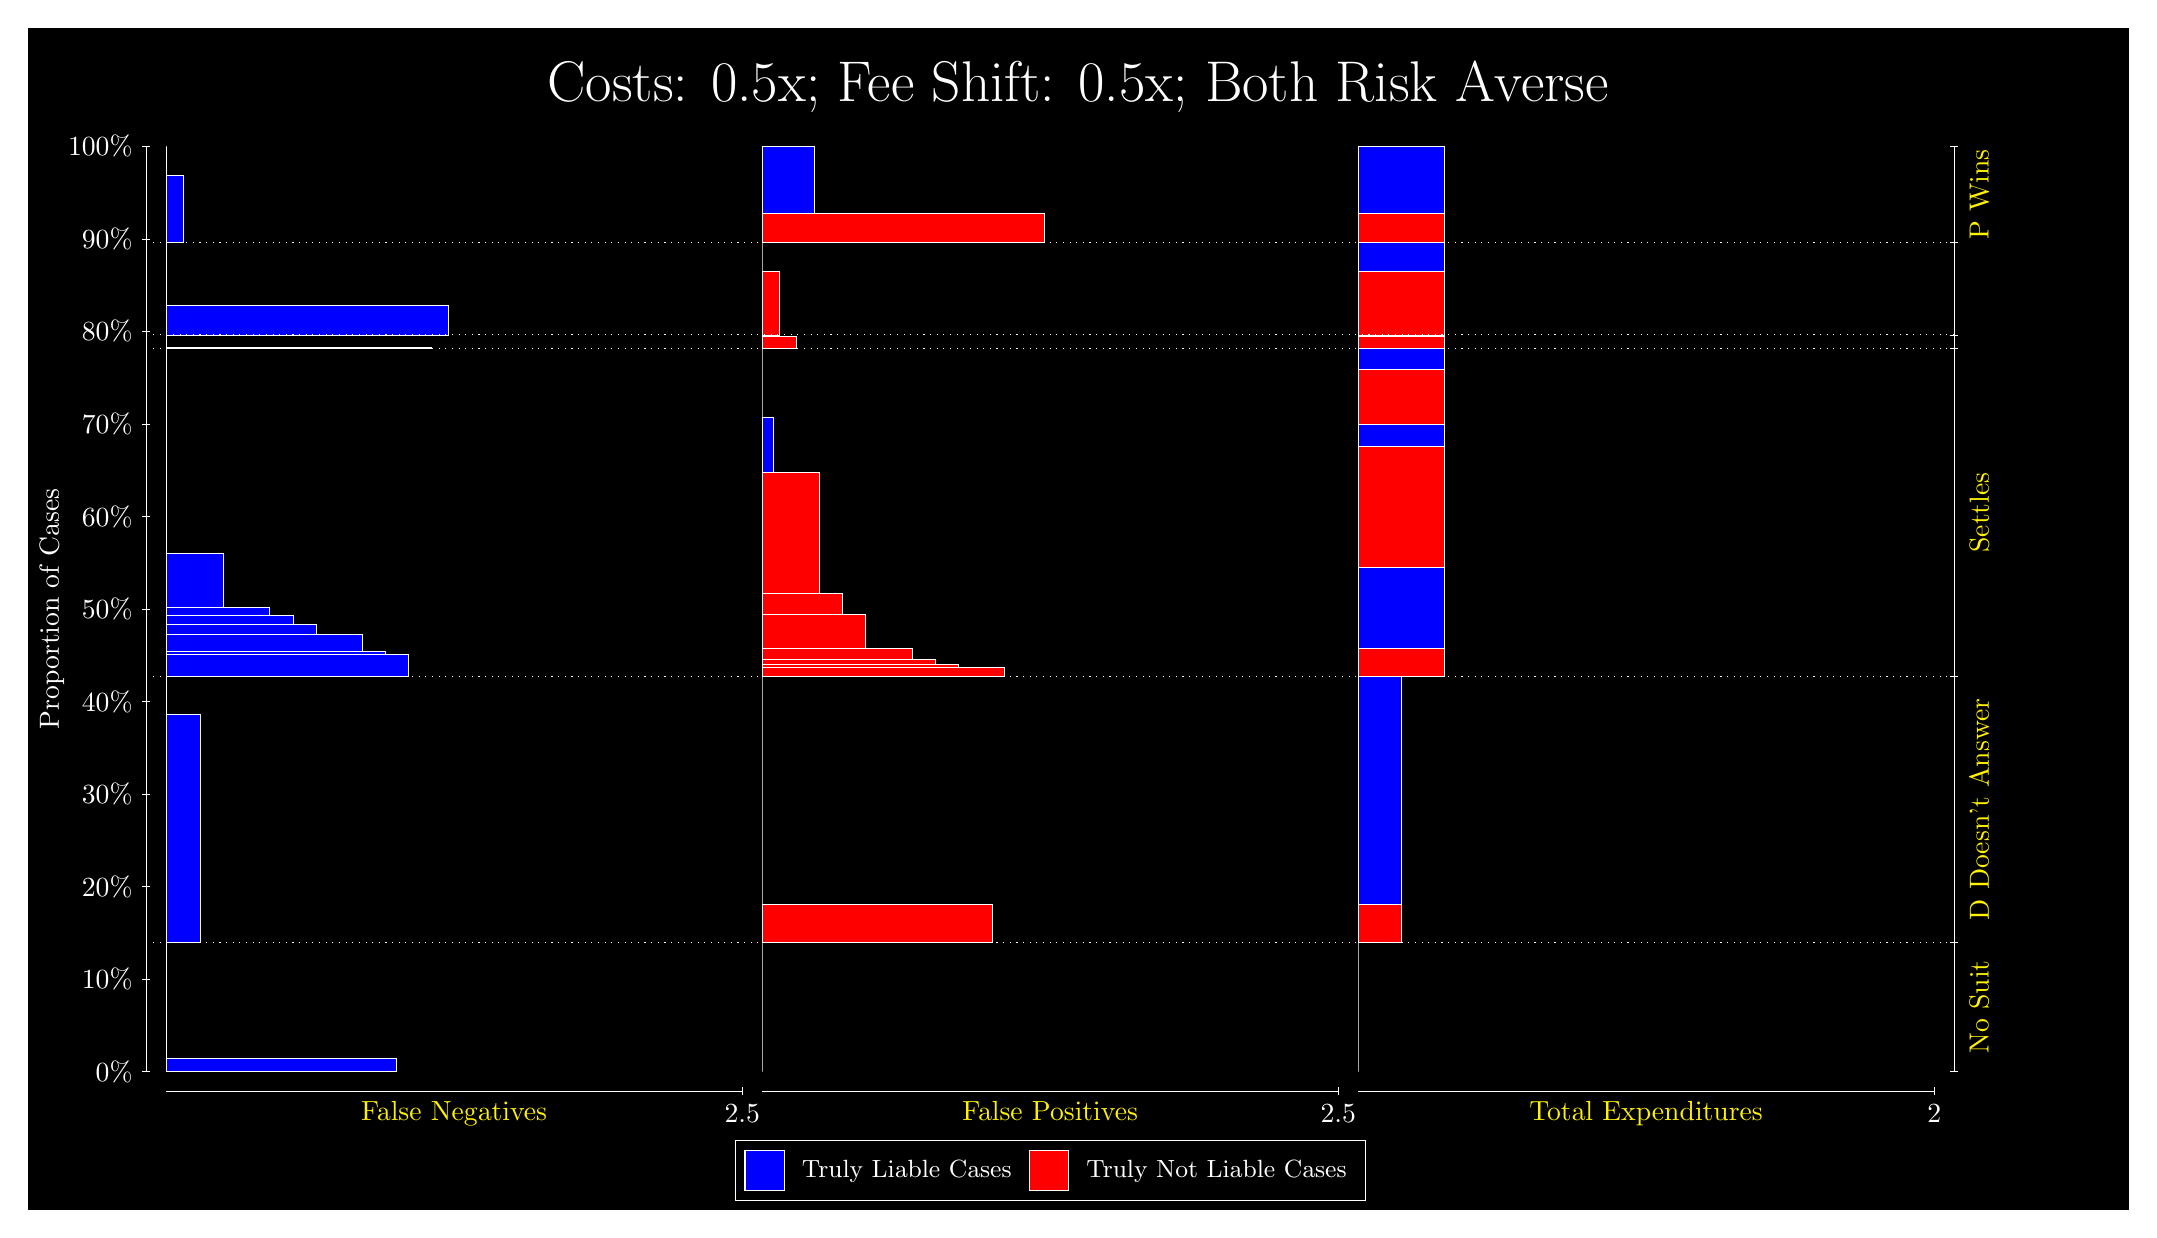
\begin{tikzpicture}
\draw[fill=black] (0,0) rectangle (26.667,15);
\draw[text=white] (0,13.5) rectangle (26.667,15) node[midway] {\huge Costs: 0.5x; Fee Shift: 0.5x; Both Risk Averse};
\draw[white, very thin] (1.5,1.75) -- (1.5,13.5);
\node[rotate=90, text=white, anchor=center] at (0.3, 7.625) {Proportion of Cases};
\draw[white, very thin] (1.45,1.75) -- (1.55,1.75);
\node[text=white, anchor=east] at (1.45, 1.75) {0\%};
\draw[white, very thin] (1.45,2.925) -- (1.55,2.925);
\node[text=white, anchor=east] at (1.45, 2.925) {10\%};
\draw[white, very thin] (1.45,4.1) -- (1.55,4.1);
\node[text=white, anchor=east] at (1.45, 4.1) {20\%};
\draw[white, very thin] (1.45,5.275) -- (1.55,5.275);
\node[text=white, anchor=east] at (1.45, 5.275) {30\%};
\draw[white, very thin] (1.45,6.45) -- (1.55,6.45);
\node[text=white, anchor=east] at (1.45, 6.45) {40\%};
\draw[white, very thin] (1.45,7.625) -- (1.55,7.625);
\node[text=white, anchor=east] at (1.45, 7.625) {50\%};
\draw[white, very thin] (1.45,8.8) -- (1.55,8.8);
\node[text=white, anchor=east] at (1.45, 8.8) {60\%};
\draw[white, very thin] (1.45,9.975) -- (1.55,9.975);
\node[text=white, anchor=east] at (1.45, 9.975) {70\%};
\draw[white, very thin] (1.45,11.15) -- (1.55,11.15);
\node[text=white, anchor=east] at (1.45, 11.15) {80\%};
\draw[white, very thin] (1.45,12.325) -- (1.55,12.325);
\node[text=white, anchor=east] at (1.45, 12.325) {90\%};
\draw[white, very thin] (1.45,13.5) -- (1.55,13.5);
\node[text=white, anchor=east] at (1.45, 13.5) {100\%};

\draw[white, very thin] (24.457,1.75) -- (24.457,13.5);
\draw[white, very thin] (24.407,1.75) -- (24.507,1.75);
\node[anchor=west] at (24.407, 1.75) {};
\draw[white, very thin] (24.407,3.3897) -- (24.507,3.3897);
\node[anchor=west] at (24.407, 3.3897) {};
\draw[white, very thin] (24.407,6.7688) -- (24.507,6.7688);
\node[anchor=west] at (24.407, 6.7688) {};
\draw[white, very thin] (24.407,10.929) -- (24.507,10.929);
\node[anchor=west] at (24.407, 10.929) {};
\draw[white, very thin] (24.407,11.105) -- (24.507,11.105);
\node[anchor=west] at (24.407, 11.105) {};
\draw[white, very thin] (24.407,12.281) -- (24.507,12.281);
\node[anchor=west] at (24.407, 12.281) {};
\draw[white, very thin] (24.407,13.5) -- (24.507,13.5);
\node[anchor=west] at (24.407, 13.5) {};

\draw[white, very thin, fill=blue] (1.75,1.75) rectangle (4.6775,1.9225);
\draw[white, very thin, fill=red] (1.75,1.9225) rectangle (1.75,3.3897);
\draw[white, very thin, fill=blue] (1.75,3.3897) rectangle (2.1891,6.2864);
\draw[white, very thin, fill=red] (1.75,6.2864) rectangle (1.75,6.7688);
\draw[white, very thin, fill=blue] (1.75,6.7688) rectangle (4.8239,7.0435);
\draw[white, very thin, fill=blue] (1.75,7.0435) rectangle (4.5312,7.0907);
\draw[white, very thin, fill=blue] (1.75,7.0907) rectangle (4.2384,7.3036);
\draw[white, very thin, fill=blue] (1.75,7.3036) rectangle (3.6529,7.4289);
\draw[white, very thin, fill=blue] (1.75,7.4289) rectangle (3.3602,7.5469);
\draw[white, very thin, fill=blue] (1.75,7.5469) rectangle (3.0674,7.6407);
\draw[white, very thin, fill=blue] (1.75,7.6407) rectangle (2.4819,8.3363);
\draw[white, very thin, fill=red] (1.75,8.3363) rectangle (1.75,10.929);
\draw[white, very thin, fill=blue] (1.75,10.929) rectangle (5.1167,10.948);
\draw[white, very thin, fill=red] (1.75,10.948) rectangle (1.75,11.105);
\draw[white, very thin, fill=blue] (1.75,11.105) rectangle (5.3362,11.475);
\draw[white, very thin, fill=red] (1.75,11.475) rectangle (1.75,12.281);
\draw[white, very thin, fill=blue] (1.75,12.281) rectangle (1.9696,13.129);
\draw[white, very thin, fill=red] (1.75,13.129) rectangle (1.75,13.5);
\draw[white, very thin, fill=red] (9.3189,1.75) rectangle (9.3189,3.2172);
\draw[white, very thin, fill=blue] (9.3189,3.2172) rectangle (9.3189,3.3897);
\draw[white, very thin, fill=red] (9.3189,3.3897) rectangle (12.246,3.8721);
\draw[white, very thin, fill=blue] (9.3189,3.8721) rectangle (9.3189,6.7688);
\draw[white, very thin, fill=red] (9.3189,6.7688) rectangle (12.393,6.8789);
\draw[white, very thin, fill=red] (9.3189,6.8789) rectangle (11.807,6.9214);
\draw[white, very thin, fill=red] (9.3189,6.9214) rectangle (11.515,6.9881);
\draw[white, very thin, fill=red] (9.3189,6.9881) rectangle (11.222,7.1215);
\draw[white, very thin, fill=red] (9.3189,7.1215) rectangle (10.636,7.5537);
\draw[white, very thin, fill=red] (9.3189,7.5537) rectangle (10.344,7.8246);
\draw[white, very thin, fill=red] (9.3189,7.8246) rectangle (10.051,9.3611);
\draw[white, very thin, fill=blue] (9.3189,9.3611) rectangle (9.4652,10.057);
\draw[white, very thin, fill=blue] (9.3189,10.057) rectangle (9.3189,10.929);
\draw[white, very thin, fill=red] (9.3189,10.929) rectangle (9.758,11.085);
\draw[white, very thin, fill=blue] (9.3189,11.085) rectangle (9.3189,11.105);
\draw[white, very thin, fill=red] (9.3189,11.105) rectangle (9.5384,11.91);
\draw[white, very thin, fill=blue] (9.3189,11.91) rectangle (9.3189,12.281);
\draw[white, very thin, fill=red] (9.3189,12.281) rectangle (12.905,12.651);
\draw[white, very thin, fill=blue] (9.3189,12.651) rectangle (9.9776,13.5);
\draw[white, very thin, fill=red] (16.888,1.75) rectangle (16.888,3.2172);
\draw[white, very thin, fill=blue] (16.888,3.2172) rectangle (16.888,3.3897);
\draw[white, very thin, fill=red] (16.888,3.3897) rectangle (17.437,3.8721);
\draw[white, very thin, fill=blue] (16.888,3.8721) rectangle (17.437,6.7688);
\draw[white, very thin, fill=red] (16.888,6.7688) rectangle (17.986,7.1215);
\draw[white, very thin, fill=blue] (16.888,7.1215) rectangle (17.986,8.1542);
\draw[white, very thin, fill=red] (16.888,8.1542) rectangle (17.986,9.6908);
\draw[white, very thin, fill=blue] (16.888,9.6908) rectangle (17.986,9.9654);
\draw[white, very thin, fill=red] (16.888,9.9654) rectangle (17.986,10.668);
\draw[white, very thin, fill=blue] (16.888,10.668) rectangle (17.986,10.929);
\draw[white, very thin, fill=red] (16.888,10.929) rectangle (17.986,11.085);
\draw[white, very thin, fill=blue] (16.888,11.085) rectangle (17.986,11.105);
\draw[white, very thin, fill=red] (16.888,11.105) rectangle (17.986,11.91);
\draw[white, very thin, fill=blue] (16.888,11.91) rectangle (17.986,12.281);
\draw[white, very thin, fill=red] (16.888,12.281) rectangle (17.986,12.651);
\draw[white, very thin, fill=blue] (16.888,12.651) rectangle (17.986,13.5);
\draw[white, dotted] (1.5,3.3897) -- (24.457,3.3897);
\draw[white, dotted] (1.5,6.7688) -- (24.457,6.7688);
\draw[white, dotted] (1.5,10.929) -- (24.457,10.929);
\draw[white, dotted] (1.5,11.105) -- (24.457,11.105);
\draw[white, dotted] (1.5,12.281) -- (24.457,12.281);
\draw[white, very thin] (1.75,1.5) -- (9.0689,1.5);
\node[text=yellow, anchor=north] at (5.4094, 1.5) {False Negatives};
\draw[white, very thin] (9.0689,1.45) -- (9.0689,1.55);
\node[text=white, anchor=north] at (9.0689, 1.45) {2.5};

\draw[white, very thin] (9.3189,1.5) -- (16.638,1.5);
\node[text=yellow, anchor=north] at (12.978, 1.5) {False Positives};
\draw[white, very thin] (16.638,1.45) -- (16.638,1.55);
\node[text=white, anchor=north] at (16.638, 1.45) {2.5};

\draw[white, very thin] (16.888,1.5) -- (24.207,1.5);
\node[text=yellow, anchor=north] at (20.547, 1.5) {Total Expenditures};
\draw[white, very thin] (24.207,1.45) -- (24.207,1.55);
\node[text=white, anchor=north] at (24.207, 1.45) {2};

\node[text=yellow, centered, rotate=90] at (24.777, 2.5699) {No Suit};
\node[text=yellow, centered, rotate=90] at (24.777, 5.0793) {D Doesn't Answer};
\node[text=yellow, centered, rotate=90] at (24.777, 8.8487) {Settles};


\node[text=yellow, centered, rotate=90] at (24.777, 12.89) {P Wins};

\draw (12.978300999999998,1.5) node[draw=none] (baseCoordinate) {};
\begin{scope}[align=center]
        \matrix[scale=0.5, draw=white, below=0.5cm of baseCoordinate, nodes={draw}, column sep=0.1cm]{
            \node[rectangle, draw, minimum width=0.5cm, minimum height=0.5cm, fill=blue] {}; &
            \node[draw=none, font=\small, text=white] (B) {Truly Liable Cases}; &
            \node[rectangle, draw, minimum width=0.5cm, minimum height=0.5cm, fill=red] {}; &
            \node[draw=none, font=\small, text=white] (B) {Truly Not Liable Cases}; \\
            };
\end{scope}

\end{tikzpicture}
\end{document}